%%%%%%%%%%%%%%%%%%%%%%%%%%%%%%%%%%%%%%%%%
% Beamer Presentation
% LaTeX Template
% Version 1.0 (10/11/12)
%
% This template has been downloaded from:
% http://www.LaTeXTemplates.com
%
% License:
% CC BY-NC-SA 3.0 (http://creativecommons.org/licenses/by-nc-sa/3.0/)
%
%%%%%%%%%%%%%%%%%%%%%%%%%%%%%%%%%%%%%%%%%

%----------------------------------------------------------------------------------------
%	PACKAGES AND THEMES
%----------------------------------------------------------------------------------------
\documentclass{beamer}

\mode<presentation> {

% The Beamer class comes with a number of default slide themes
% which change the colors and layouts of slides. Below this is a list
% of all the themes, uncomment each in turn to see what they look like.

%\usetheme{default}
%\usetheme{AnnArbor}
%\usetheme{Antibes}
%\usetheme{Bergen}
%\usetheme{Berkeley}
%\usetheme{Berlin}
%\usetheme{Boadilla}
%\usetheme{CambridgeUS}
%\usetheme{Copenhagen}
%\usetheme{Darmstadt}
%\usetheme{Dresden}
%\usetheme{Frankfurt}
%\usetheme{Goettingen}
%\usetheme{Hannover}
%\usetheme{Ilmenau}
%\usetheme{JuanLesPins}
%\usetheme{Luebeck}
\usetheme{Madrid}
%\usetheme{Malmoe}
%\usetheme{Marburg}
%\usetheme{Montpellier}
%\usetheme{PaloAlto}
%\usetheme{Pittsburgh}
%\usetheme{Rochester}
%\usetheme{Singapore}
%\usetheme{Szeged}
%\usetheme{Warsaw}

% As well as themes, the Beamer class has a number of color themes
% for any slide theme. Uncomment each of these in turn to see how it
% changes the colors of your current slide theme.

%\usecolortheme{albatross}
%\usecolortheme{beaver}
%\usecolortheme{beetle}
%\usecolortheme{crane}
%\usecolortheme{dolphin}
%\usecolortheme{dove}
%\usecolortheme{fly}
%\usecolortheme{lily}
%\usecolortheme{orchid}
%\usecolortheme{rose}
%\usecolortheme{seagull}
%\usecolortheme{seahorse}
%\usecolortheme{whale}
%\usecolortheme{wolverine}

%\setbeamertemplate{footline} % To remove the footer line in all slides uncomment this line
%\setbeamertemplate{footline}[page number] % To replace the footer line in all slides with a simple slide count uncomment this line

%\setbeamertemplate{navigation symbols}{} % To remove the navigation symbols from the bottom of all slides uncomment this line
}

\usepackage{graphicx} % Allows including images
\usepackage{booktabs} % Allows the use of \toprule, \midrule and \bottomrule in tables

% Eigen packages
\usepackage[dutch]{babel}
\usepackage{multirow}

\usepackage[style=apa,backend=biber]{biblatex}
\DeclareLanguageMapping{dutch}{dutch-apa}

\usepackage[font=scriptsize,justification=centering]{caption}
\usepackage{filecontents}
\usepackage{textcomp}

% Bibliografie (afbeeldingen etc.)
\begin{filecontents}{\jobname.bib}
@Conference{KendiOnbekend,
  Title                    = {ZFS: Enhancing the Open Source Storage System (and the Kernel)},
  Author                   = {Kendi, Christian},
  Year                     = {Onbekend},
  Language                 = {English},
  Url                      = {https://www.blackhat.com/presentations/bh-dc-10/Kendi_Christian/Blackhat-DC-2010-Kendi-Enhancing-ZFS-slides.pdf},
  Owner                    = {Jonas De Moor},
  Timestamp                = {25.04.2017}}

@Techreport{ZFSBonwick,
  Title                    = {The Zettabyte Filesystem},
  Author                   = {Bonwick, Jeff and others},
  Year                     = {2002},
  Language                 = {English},
  Month                    = {Unknown},
  Url                      = {http://citeseerx.ist.psu.edu/viewdoc/download?doi=10.1.1.184.3704&rep=rep1&type=pdf},
  Organization             = {Sun Microsystems},
  Owner                    = {Jonas De Moor},
  Timestamp                = {25.04.2017}}

@Techreport{Microsystems2006,
  Title                    = {ZFS on-disk specification},
  Author                   = {{Sun Microsystems}},
  Year                     = {2006},
  Language                 = {English},
  Url                      = {http://www.giis.co.in/Zfs_ondiskformat.pdf},

  Owner                    = {Jonas De Moor},
  Timestamp                = {25.04.2017}}
\end{filecontents}

\renewcommand*{\nameyeardelim}{\addcomma\addspace}

\addbibresource{\jobname.bib}

%----------------------------------------------------------------------------------------
%	TITLE PAGE
%----------------------------------------------------------------------------------------

\title[Presentatie Bachelorproef]{ZFS met RAID-Z als alternatief voor klassieke RAID-oplossingen} % The short title appears at the bottom of every slide, the full title is only on the title page

\author{Jonas De Moor} % Your name
\institute[HoGent] % Your institution as it will appear on the bottom of every slide, may be shorthand to save space
{
Toegepaste Informatica - Systeem- en Netwerkbeheer \\ Hogeschool Gent \\ % Your institution for the title page
\medskip
\textit{jonas.demoor.v3741@student.hogent.be} % Your email address
}
\date{\today} % Date, can be changed to a custom date

\begin{document}

\begin{frame}
\titlepage % Print the title page as the first slide
\end{frame}

\begin{frame}
\frametitle{Inhoud} % Table of contents slide, comment this block out to remove it
\tableofcontents % Throughout your presentation, if you choose to use \section{} and \subsection{} commands, these will automatically be printed on this slide as an overview of your presentation
\end{frame}

%----------------------------------------------------------------------------------------
%	PRESENTATION SLIDES
%----------------------------------------------------------------------------------------

%------------------------------------------------
\section{Achtergrond} % Sections can be created in order to organize your presentation into discrete blocks, all sections and subsections are automatically printed in the table of contents as an overview of the talk
%------------------------------------------------

\subsection{Motivatie} % A subsection can be created just before a set of slides with a common theme to further break down your presentation into chunks

%------------------------------------------------

\begin{frame}
\frametitle{Motivatie voor het voeren van dit onderzoek}

  \begin{itemize}
    \item{RAID5 'write hole'}
    \item Relatie tussen BTRFS en ZFS
    \item ZFS On Linux (cf. Ubuntu 16.04 LTS)
    \item Interesses: Linux en Unix
  \end{itemize}

\end{frame}

%------------------------------------------------

\subsection{Onderzoeksvragen}

%------------------------------------------------

\begin{frame}
  \frametitle{Onderzoeksvragen}
  \begin{itemize}
	  \item Wat zijn de grootste verschillen tussen een klassieke RAID-oplossing en ZFS RAID-Z?
	  \item Hoe is de architectuur van ZFS opgebouwd en op welke manieren tracht het oplossingen te vinden voor de problemen die zich voordoen bij andere bestandssystemen en RAID-opstellingen?
    \item Hoe staat het met data-integriteit en performantie\footnote{Met 'performantie' wordt het aantal I/O's per seconde en de globale CPU-belasting bedoeld.} bij ZFS onder verschillende workloads en toepassingen?
  \end{itemize}
\end{frame}

%------------------------------------------------

\subsection{Opbouw van het onderzoek}

%------------------------------------------------

\begin{frame}
\frametitle{Opbouw van het onderzoek}

Twee grote onderdelen:
  \begin{enumerate}
    \item Theoretisch gedeelte
      \begin{itemize}
        \item Inleiding tot RAID-niveaus
        \item Architectuur en ontwerpprincipes van ZFS
        \item Interne datastructuren en transactiemodel
      \end{itemize}
    \item{Praktisch gedeelte}
      \begin{itemize}
        \item Storage Pools \& VDEV's
        \item Datasets
        \item Performantie \& Betrouwbaarheid
      \end{itemize}
  \end{enumerate}
\end{frame}

%------------------------------------------------

\subsection{Gehanteerde methodiek}

%------------------------------------------------

\begin{frame}
\frametitle{Gehanteerde methodiek}
  \begin{itemize}
    \item Phoronix Benchmark: performantietesten op fysieke machine
    \begin{itemize}
      \item FIO (Flexible I/O Tester): IOPS
      \item FS-Mark: bestandssysteemoperaties
      \item PostMark: simulatie van webserver/mailserver
      \item SQLite: databankoperaties
    \end{itemize}
    \item Virtuele Machine: betrouwbaarheidstesten
    \begin{itemize}
      \item Wegvallen van een schijf (array van drie schijven)
      \item Dataverlies door gebruikersfout
      \item Bescherming tegen datacorruptie
    \end{itemize}
  \end{itemize}
\end{frame}

\begin{frame}
  \frametitle{Gehanteerde methodiek}
  \begin{table}
    \centering
    \begin{tabular}{c l}
      \toprule
      \multicolumn{2}{c}{\textbf{Specificaties}} \\ 
      \midrule
      \textbf{Fabrikant} & HP \\
      \hline
      \textbf{Model} & HP Pavilion Elite HPE-310be \\
      \hline
      \textbf{CPU} & Intel Core i5 650 @ 3.2 GHz (2 Cores; 4 Threads) \\
      \hline
      \textbf{Geheugen} & 10GB DDR3 @ 1333MHz \\ 
      \hline
      \textbf{GPU} & AMD Radeon HD 5570 \\
      \hline
      \multirow{4}{*}{\textbf{Interne schijven}} & SAMSUNG HD103SJ (1TB) \\
        & WDC WD1002FAEX-0 (1TB) \\
        & WDC WD5000AZRX-0 (500GB) \\
      \hline
      \textbf{Externe schijf} & WD Elements 1078 (1TB) \\
      \hline
      \textbf{RAID Controller} & Intel Corporation SATA RAID Controller \\
      \bottomrule
    \end{tabular}
    \caption{Specificaties van het fysieke systeem dat gebruikt werd doorheen de bachelorproef (data verkregen via \texttt{lshw})}
    \label{tab:specs_desktop }
  \end{table}

\end{frame}

\begin{frame}
  \frametitle{Gehanteerde methodiek}
  \begin{table}[h]
    \centering
    \begin{tabular}{c l}
      \toprule
      \multicolumn{2}{c}{\textbf{Specificaties Virtuele Machine}} \\
      \hline
      \textbf{OS} & Fedora Server 25 \\
      \hline
      \textbf{CPU} & 4x Host CPU (Intel Core i7-4712HQ CPU @ 2.30GHz) \\
      \hline
      \textbf{Geheugen} & 8GB \\
      \hline
      \textbf{OS-schijf} & 20GB (\texttt{/dev/sda}; SATA non-hot-pluggable) \\
      \hline
      \multirow{4}{*}{\textbf{Zpool schijven}} & 40GB (\texttt{/dev/sdb}; SATA hot-pluggable) \\
        & 40GB (\texttt{/dev/sdc}; SATA hot-pluggable) \\
        & 40GB (\texttt{/dev/sdd}; SATA hot-pluggable) \\
      \hline
      \multirow{2}{*}{\textbf{NIC's}} & VirtualBox NAT-adapter (10.0.2.15/24) \\
        & VirtualBox Host-only Adapter (192.168.56.10/24) \\
      \bottomrule
    \end{tabular}
    \caption{Specificaties van de virtuele machine die gebruikt werd voor de betrouwbaarheidstesten}
    \label{tab:specs_vm}
  \end{table}
\end{frame}

\begin{frame}
  \frametitle{Inhoud} % Table of contents slide, comment this block out to remove it
  \tableofcontents % Throughout your presentation, if you choose to use \section{} and \subsection{} commands, these will automatically be printed on this slide as an overview of your presentation
\end{frame}

%------------------------------------------------
\section{Onderzoek}
%------------------------------------------------

\subsection{Achtergrondinformatie m.b.t. ZFS}

%------------------------------------------------

\begin{frame}
\frametitle{ZFS: een kort overzicht}
\begin{itemize}
  \item Copy-On-Write bestandssysteem
  \item Ontwikkeld door Sun Microsystems (begin jaren 2000) 
  \item Oorspronkelijk onderdeel van Solaris
  \item Nu: verdere ontwikkeling via OpenZFS (en Oracle)
  \item Ondertussen ook beschikbaar op BSD en Linux (ZFS on Linux)
  \item{Beschikt over RAID-Z (softwarematige RAID)}
\end{itemize}
\end{frame}

%------------------------------------------------

\subsection{Architectuur van ZFS}

%------------------------------------------------

\begin{frame}
\frametitle{Architectuur van ZFS}
  \begin{figure}
    \centering
    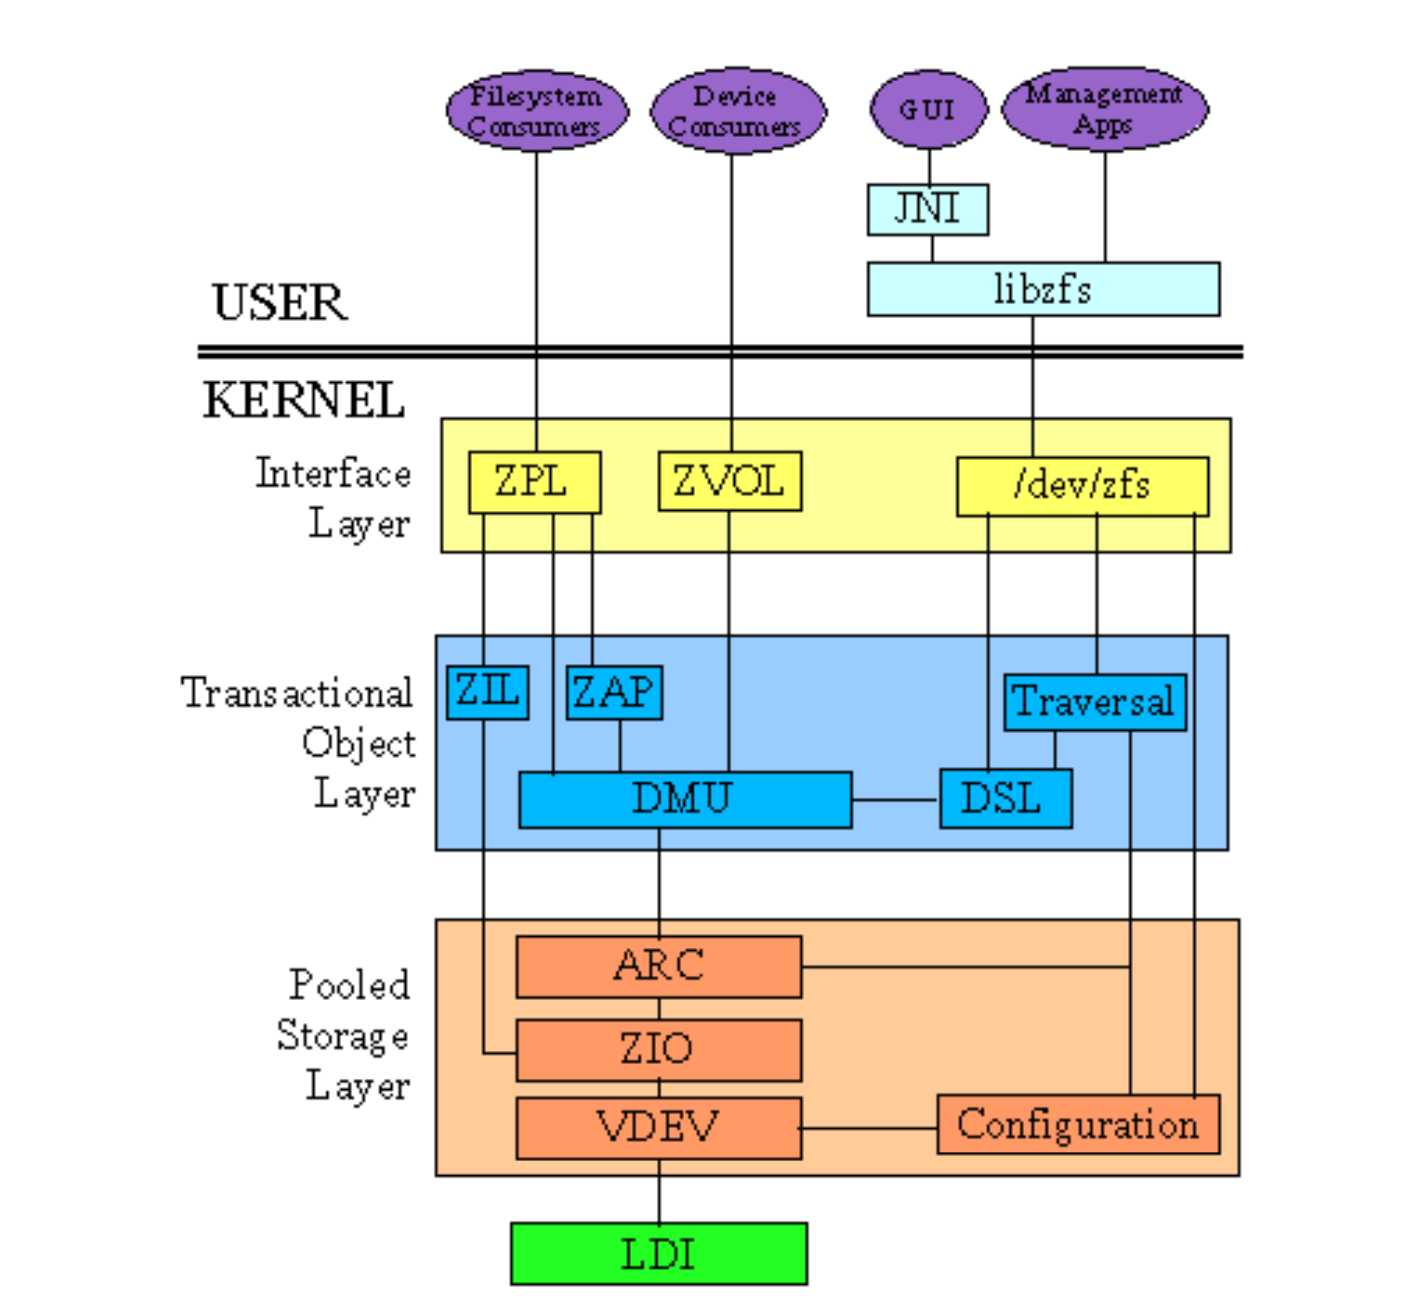
\includegraphics[width=0.63\linewidth]{img/h3-zfs_overview}
    \caption{Een overzicht van de verschillende componenten van ZFS \autocite{KendiOnbekend}}
    \label{fig:kendi_zfs_overview}
  \end{figure}
\end{frame}

\begin{frame}
  \frametitle{Architectuur van ZFS}
  \begin{figure}
    \centering
    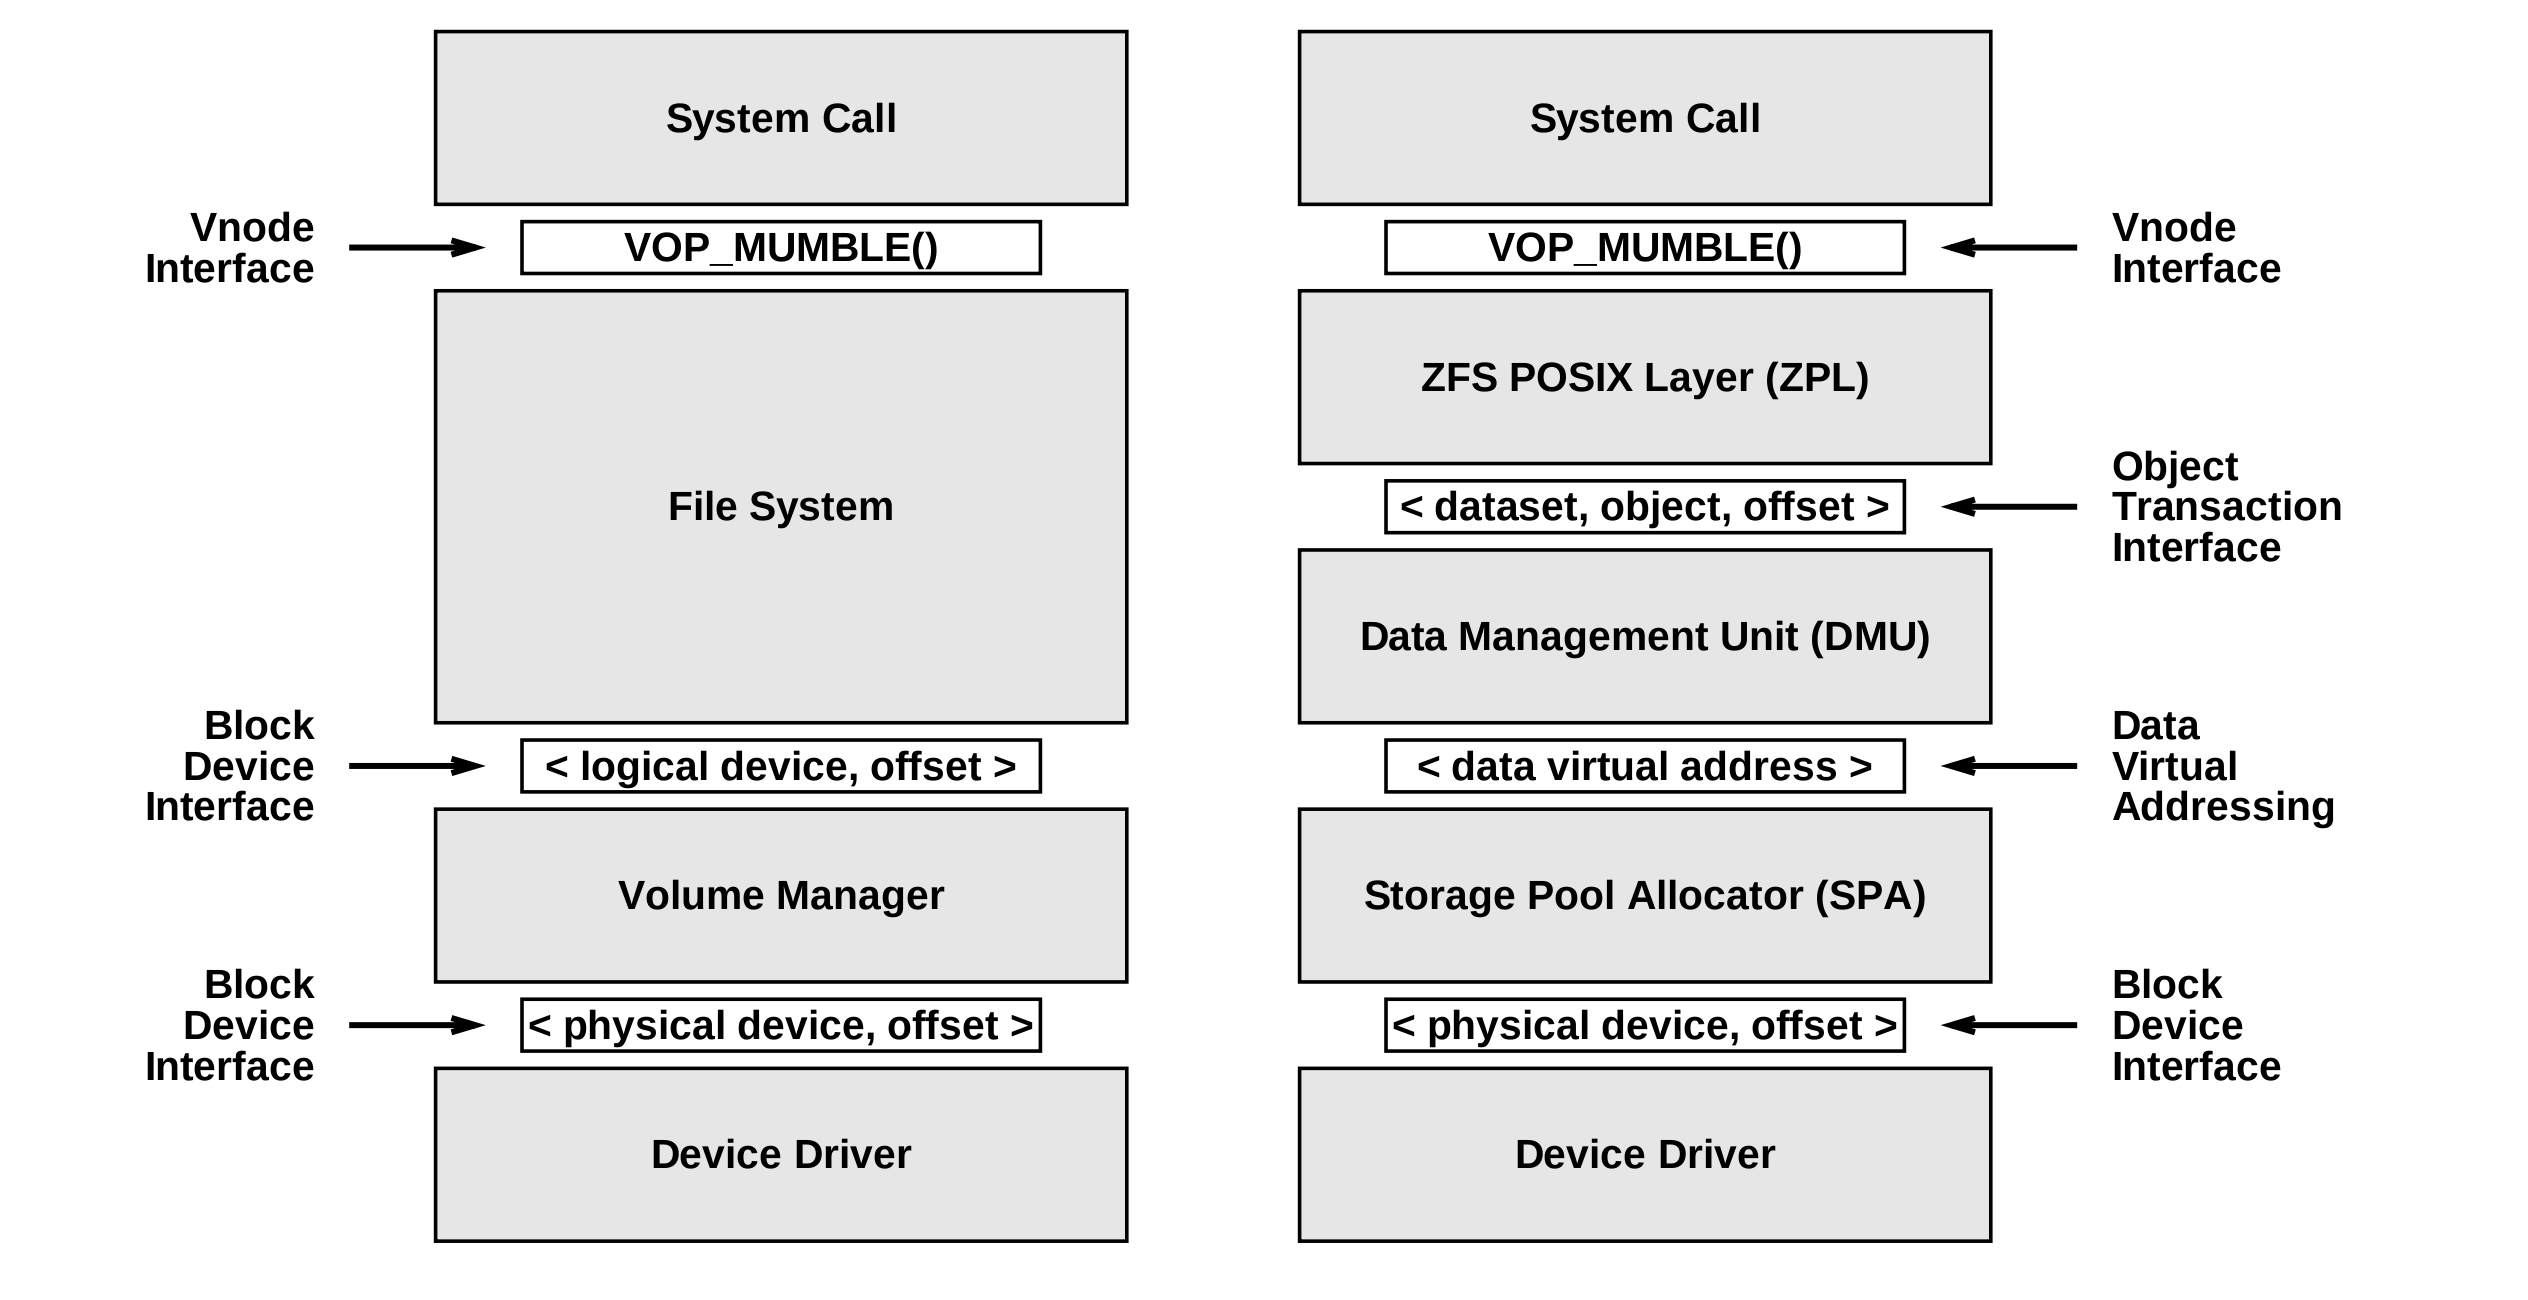
\includegraphics[width=\linewidth]{img/bs-vs-zfs}
    \caption{Vergelijking tussen een 'traditionele' storage stack (links) en de ZFS storage stack (rechts) \autocite{ZFSBonwick}}
    \label{fig:bonwick_zfs_vs_fs}
  \end{figure}
\end{frame}

%------------------------------------------------

\subsection{VDEV's \& Storage Pools}

%------------------------------------------------

\begin{frame}
  \frametitle{Storage Pools}
  \begin{itemize}
    \item Abstractie voor fysieke apparaten \textbf{\textrightarrow} gegroepeerd in VDEV's
    \item Dynamische allocatie van opslagruimte
    \item Schijven kunnen worden toegevoegd zonder downtime\footnote{Afhankelijk van de situatie}    
  \end{itemize}

  \begin{figure}
    \centering
    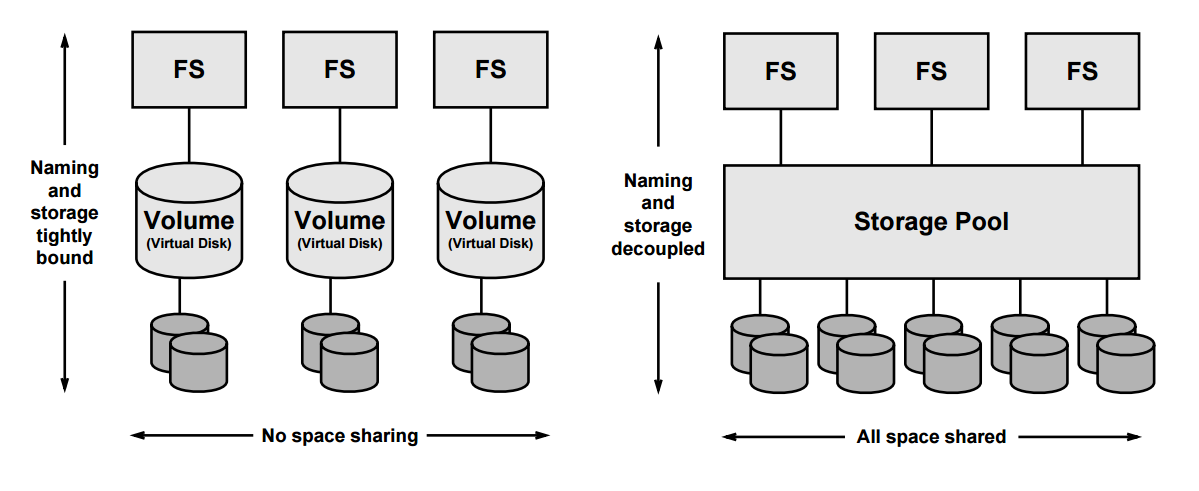
\includegraphics[width=0.8\textwidth]{img/h3-pools-vs-vols}
    \caption{Illustratie van ZFS pooled storage (rechts) t.o.v.volume-based storage (links) \autocite{ZFSBonwick}}
    \label{fig:bonwick_pools_illustratie}
    \end{figure}
\end{frame}

%------------------------------------------------

\begin{frame}
  \frametitle{VDEV's: Virtual Devices}
  \begin{itemize}
    \item Bouwstenen van storage pools
    \item RAID-niveaus binnen ZFS:
    \begin{itemize}
      \item Stripes, Mirrors, RAID-Z, etc. 
    \end{itemize}
    \item Speciale VDEV's:
    \begin{itemize}
      \item SLOG, L2ARC
    \end{itemize}
  \end{itemize}
  \begin{figure}
    \centering
    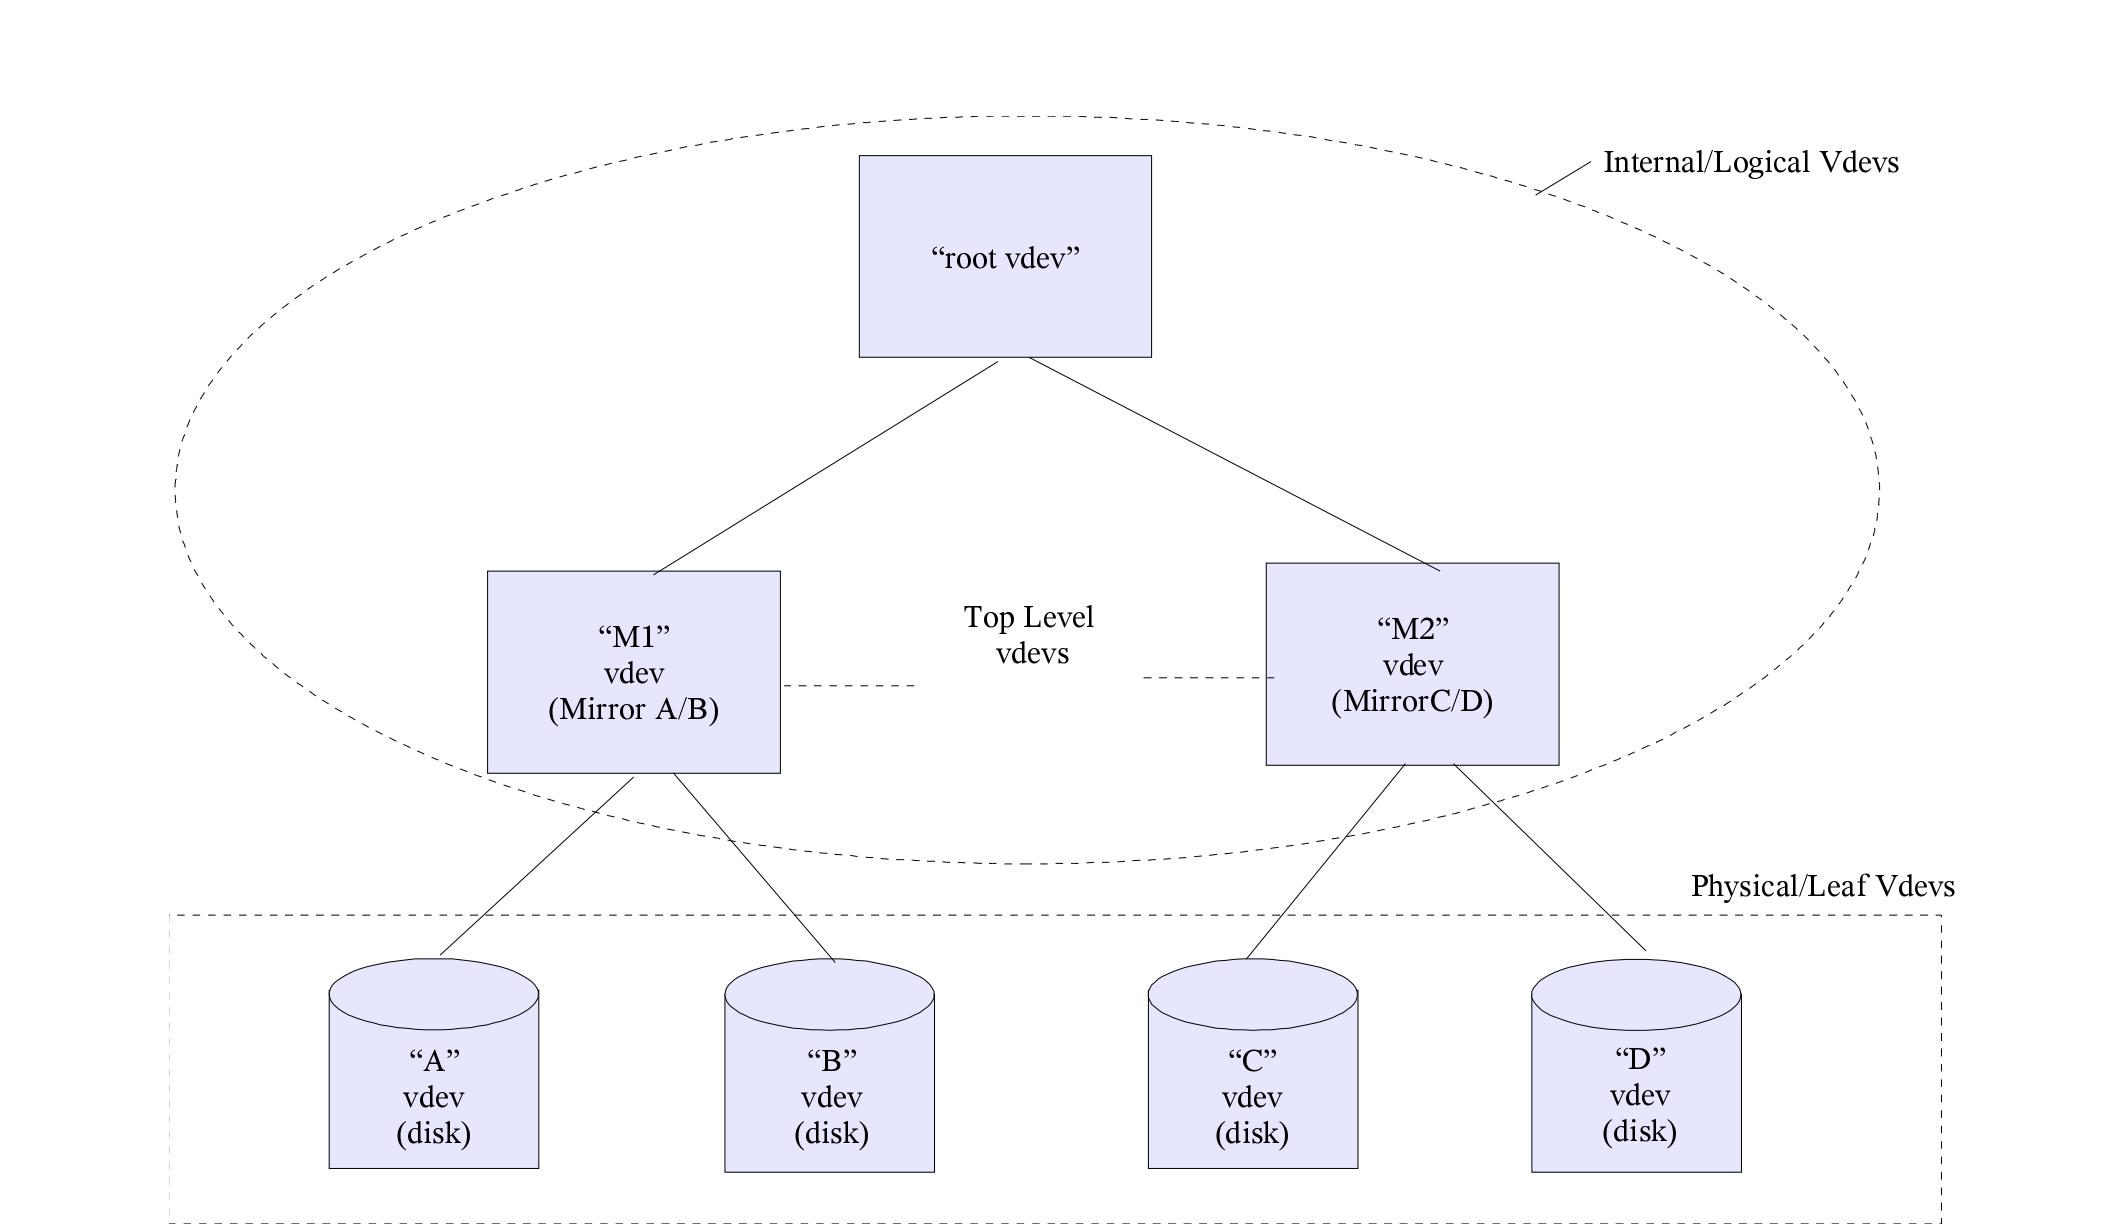
\includegraphics[width=0.6\textwidth]{img/h6_vdevs_tree}
    \caption{Conceptuele voorstelling van VDEV's in een boomstructuur \autocite{Microsystems2006}}
    \label{fig:vdevs_boom}
  \end{figure}
\end{frame}

%------------------------------------------------

\begin{frame}[fragile]
  \frametitle{Voorbeeld: zpool met een RAID-Z VDEV}
  \begin{verbatim}
    $ zpool create storage raidz1 /dev/sda /dev/sdb /dev/sdc
    $ zpool status
      pool: storage
      state: ONLINE
      scan: none requested
      config:

	    NAME        STATE     READ WRITE CKSUM
	    storage     ONLINE       0     0     0
	      raidz1-0  ONLINE       0     0     0
	        sda     ONLINE       0     0     0
	        sdb     ONLINE       0     0     0
	        sdc     ONLINE       0     0     0

      errors: No known data errors
  \end{verbatim}
\end{frame}

%------------------------------------------------

\subsection{Benchmarks}

%------------------------------------------------

\begin{frame}
  \frametitle{Inhoud}
  \tableofcontents
\end{frame}

%------------------------------------------------

\begin{frame}
  \frametitle{Benchmarks}
  FIO-benchmark: aantal IOPS (Invoer/Uitvoer-bewerkingen per seconde)
  
\end{frame}

%------------------------------------------------
\section{Conclusie}
%------------------------------------------------

%------------------------------------------------

\begin{frame}[allowframebreaks]
  \frametitle{Referenties}
  \printbibliography
\end{frame}

%------------------------------------------------

\begin{frame}
\Huge{\centerline{Zijn er nog vragen?}}
\end{frame}

%----------------------------------------------------------------------------------------

\end{document} 
